%%%%
%% Design :: Class Diagrams
%%%
\section{Class Diagrams}
\label{sec:class_diagram}

Within this section a range of class diagrams will be presented an discussed. 
``A class diagram describes the structure of a system by highlighting the 
system's classes, attributes, methods, and relationships with other classes''
\citep{lunn03}.

Figure \ref{fig:package_overview} illustrates the seven packages that make up 
the cryptic crossword solver. Over the following subsections, each of the 
packages will be described in more detail.

\begin{figure}[H]
  \centering
  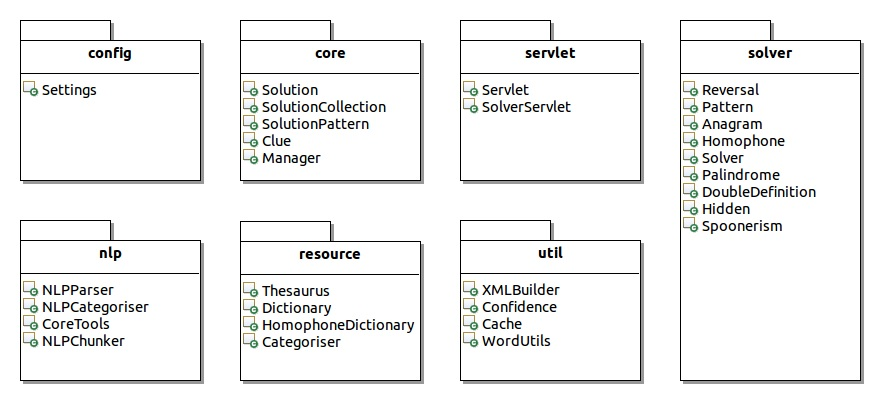
\includegraphics[width=0.9\textwidth]{design/class/package_layout.jpg}
  \caption{Package overview of the Cryptic Crossword Solver system}
  \label{fig:package_overview}
\end{figure}


%%%%
%% Design :: Class Diagrams :: Config
%%%
\subsection{Config}
\label{sub:config}

The configuration class only contains one class, Settings. The Settings class is 
designed to hold all application specific settings, and each setting can be 
altered based upon the mode it is being run under --- for example development, 
testing or production.

The Settings class follows the single design pattern which ensures that the 
class will have only one instance \citep{gof}. This prevents various numbers of
the same Settings objects being used in memory, and thus wasting valuable space.

Figure \ref{fig:config_package} illustrates the config package, containing the 
Settings class.

\begin{figure}[H]
  \centering
  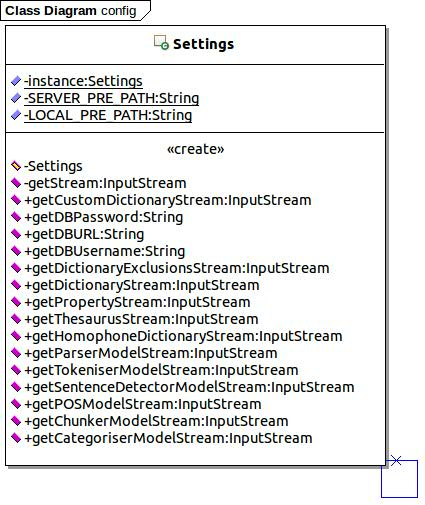
\includegraphics[width=0.5\textwidth]{design/class/config.jpg}
  \caption{Config package class diagram}
  \label{fig:config_package}
\end{figure}


%%%%
%% Design :: Class Diagrams :: Core
%%%
\subsection{Core}
\label{sub:core}

The core package contains the various classes that are deemed to be at the heart
of the system. A class has been devoted to the clue, a solution and a solution 
pattern class various specific functionality.

For example the solution pattern provides methods that allow for words to be 
computed, without having to work out the length of each word every time. The 
clue class is able to deduce the best solutions, based upon a collection of 
solutions.

The SolutionsCollection provides a simple interface to handle any number of 
solutions. The SolutionsCollection uses the HashSet as it's base class, which 
prevents duplicate solutions to be stored within the same set. It also provides
a faster lookup, in comparison to List based structures.

Finally the manager class is the heart of the system and was originally 
illustrated in the subsection \nameref{sub:solving_a_clue} on page 
\pageref{sub:solving_a_clue}. It will be able distribute a clue and it's 
solution pattern to the various solvers asynchronously. It also handles the 
merging of results within the \texttt{distributeAndSolve} method.as

Figure \ref{fig:core_package} illustrates the core package, containing the 
various core classes.

\begin{figure}[H]
  \centering
  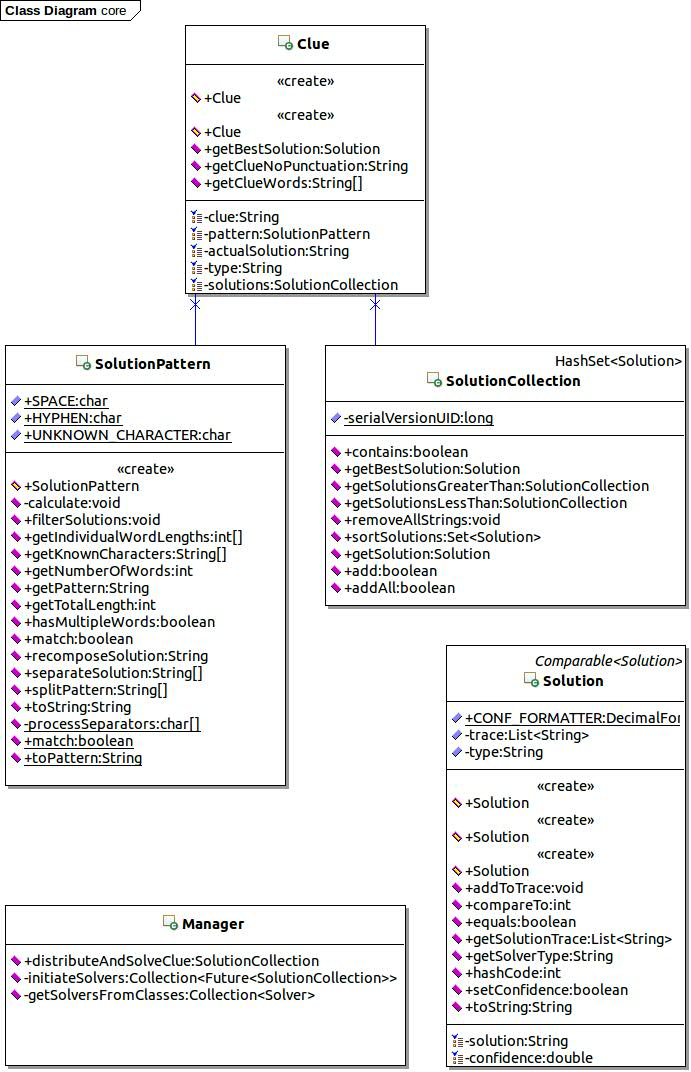
\includegraphics[width=0.8\textwidth]{design/class/core.jpg}
  \caption{Core package class diagram}
  \label{fig:core_package}
\end{figure}


%%%%
%% Design :: Class Diagrams :: NLP
%%%
\subsection{NLP}
\label{sub:nlp}

The NLP package contains the various classes that are focus on providing the 
system with an interface to the Apache OpenNLP library. This will allow the 
system to be able to use natural language processing techniques from within the 
application.

%% Additional write to be added here

Figure \ref{fig:nlp_package} illustrates the NLP package, containing the 
various NLP related classes.

\begin{figure}[H]
  \centering
  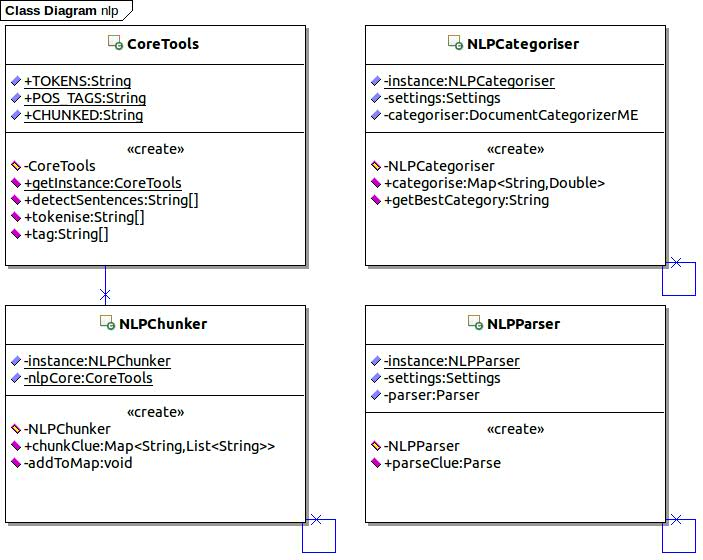
\includegraphics[width=0.9\textwidth]{design/class/nlp.jpg}
  \caption{NLP package class diagram}
  \label{fig:nlp_package}
\end{figure}


%%%%
%% Design :: Class Diagrams :: Resource
%%%
\subsection{Resource}
\label{sub:resource}

The resource package contains various classes that provide interfaces to the 
array of resources that the system will use. As with the config package, all 
classes utilise the Singleton design pattern.

The Dictionary, Thesaurus and HomophoneDictionary classes provide the 
functionality that would be expected. For example the Dictionary has the ability
to check to see if a given word is a `real word'. Where as the Thesaurus class
has the ability to find synonyms of a given word.

All of the classes are able to utilise the SolutionPattern class (as found in 
the core package), which allows for words to be matched upon various known and 
unknown character combinations.

The Categoriser class will map a given clue and solution combination to various 
lists of clue type indicators. If an indicator is found, then the confidence 
rating of the solution will be increased. This will form part of the overall 
ranking of a solution.

Figure \ref{fig:resource_package} illustrates the resource package, containing 
the various resource classes.

\begin{figure}[H]
  \centering
  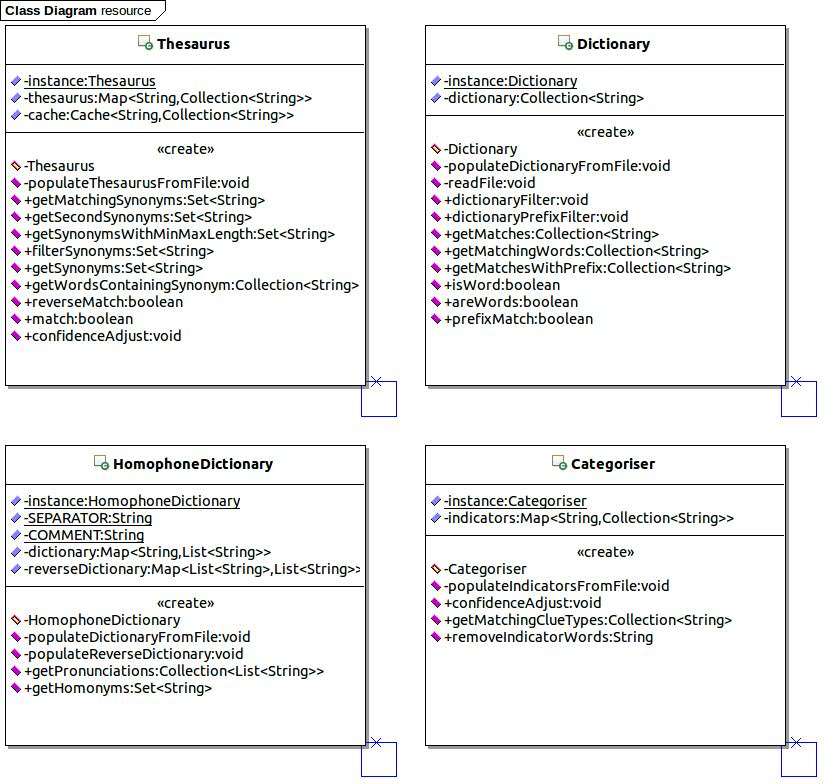
\includegraphics[width=0.9\textwidth]{design/class/resource.jpg}
  \caption{Resource package class diagram}
  \label{fig:resource_package}
\end{figure}


%%%%
%% Design :: Class Diagrams :: Servlet
%%%
\subsection{Servlet}
\label{sub:servlet}

The servlet package contains two classes that provide the web service interface.
Both classes tie into the Tomcat system, which allow provides a container for 
the website to sit in. 

The Servlet class is a custom base class that various levels of common 
functionality, that other specific classes may which to utilise. This 
functionality includes converting XML into JSON, and determining if a reject was
made via AJAX.

The Solver class extends the Servlet class, and provides the functionality 
required for handling solver related queries. All GET and POST requests to the
Solver class made via AJAX will be treated as a request over the web. 

However all GET and POST requests that do not pass the AJAX flag, will be 
treated as if the user intended on viewing a website. All non-AJAX posts will be 
redirected to the Solver's default HTML page, which will allow users to enter 
the various parameters via a web form.

It is intended that the solver class will listen upon all requests upon the 
/solver URL path --- for example \href{}{www.example.com/solver}.

Figure \ref{fig:servlet_package} illustrates the servlet package, containing 
the public web service related classes.

\begin{figure}[H]
  \centering
  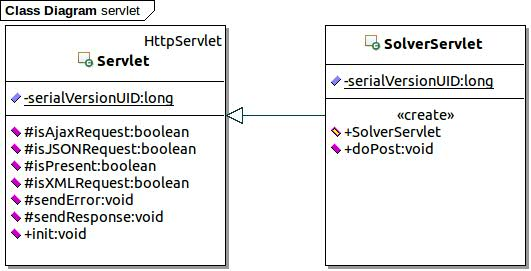
\includegraphics[width=0.6\textwidth]{design/class/servlet.jpg}
  \caption{Servlet package class diagram}
  \label{fig:servlet_package}
\end{figure}


%%%%
%% Design :: Class Diagrams :: Solver
%%%
\subsection{Solver}
\label{sub:solver}

The solver package contains the all of the solver algorithm classes that are 
used as part of the over all solving process. Each solver extends a main Solver
class which provides a number of base methods, as well as some additional 
methods that require each solver to override.

The Solver class implements the Callable interface, which provides functionality
to run a class in it's own thread. A design decision was taken that the Callable
interface was to be used, as once it has finished executing it is able to return
an object unlike similar interfaces such as Runnable.

In this case the Solver class will return a SolutionCollection object, which 
contains all the solutions that the given solver has managed to compute.

Figure \ref{fig:solver_package} illustrates the solver package, containing the
various solving algorithms used by the system.

\begin{figure}[H]
  \centering
  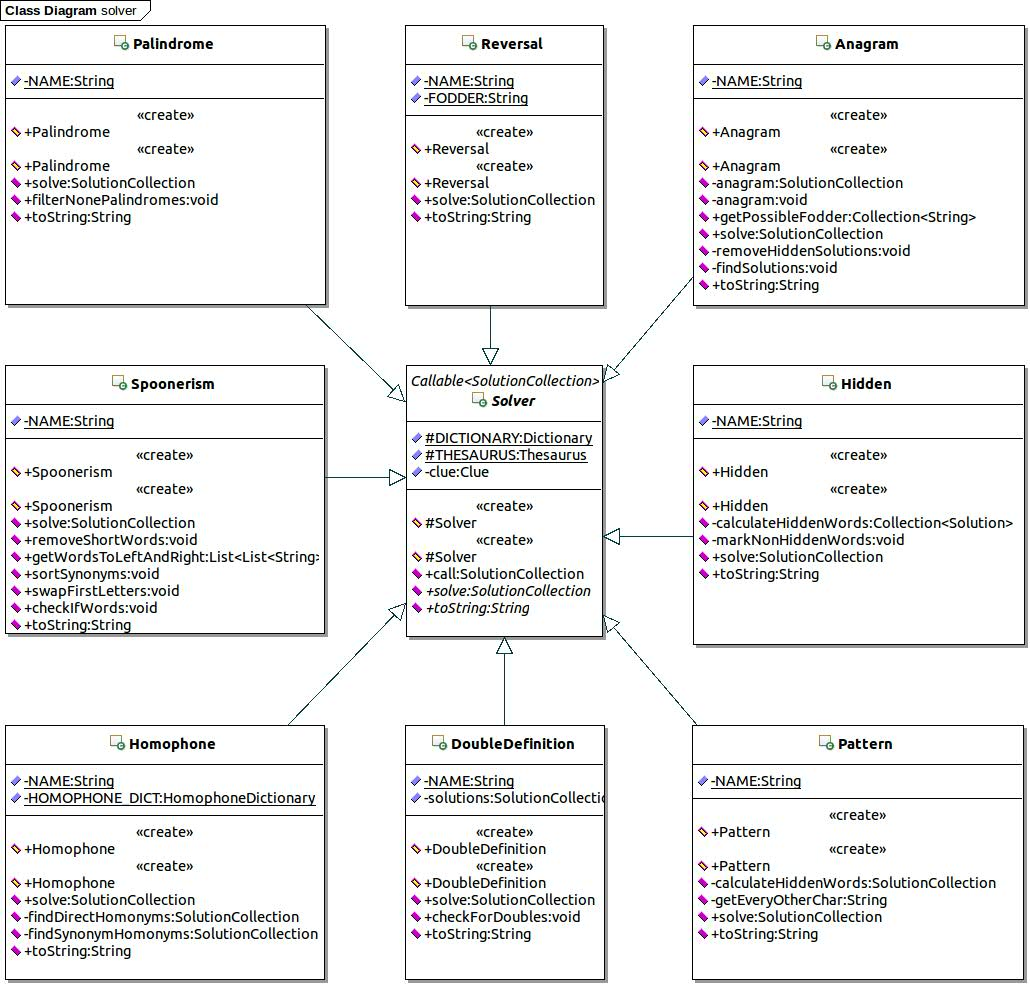
\includegraphics[width=0.9\textwidth]{design/class/solver.jpg}
  \caption{Solver package class diagram}
  \label{fig:solver_package}
\end{figure}


%%%%
%% Design :: Class Diagrams :: Util
%%%
\subsection{Util}
\label{sub:util}

The util package contains a number of classes that are unrelated with each 
other, but provide functionality that is required throughout the system.

The XMLBuilder class provides a data encapsulation layer around an XML library. 
This class is able to build well-formed XML documents that are suitable for the
system's out.

The WordUtils class provides a number of generic methods that are used to 
manipulate strings as words. This functionality is particular useful, as the 
system will be dealing with large amounts of natural language (English) 
sentences.

The confidence class provides a number of rules, that when applied to a solution
is able to deduce it's overall `correctness'. This value is directly reported 
back to the user as the confidence rating.

Figure \ref{fig:util_package} illustrates the util package, containing the
a number of additional utility classes.

\begin{figure}[H]
  \centering
  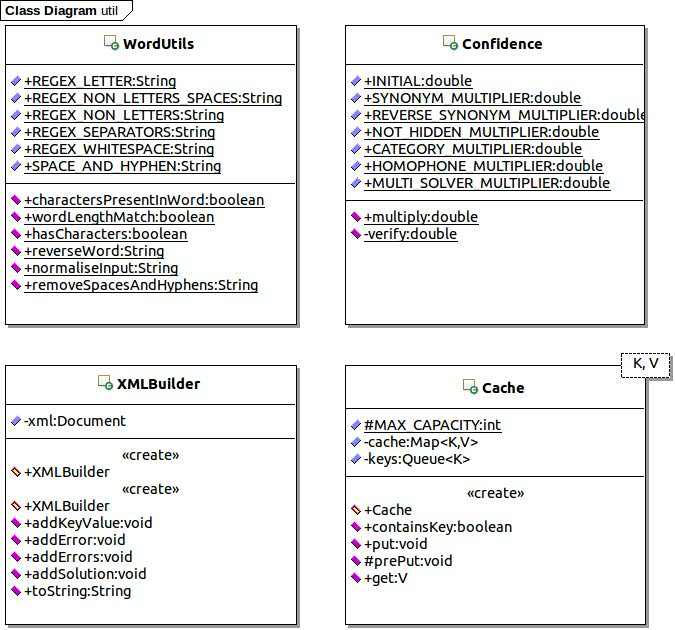
\includegraphics[width=0.8\textwidth]{design/class/util.jpg}
  \caption{Util package class diagram}
  \label{fig:util_package}
\end{figure}
